A detailed knowledge of the wave motion in all locations is generally not required, 
one may rather be interested in the evolution of some wave properties on distances 
much larger than the wavelength.  A statistical approach is therefore preferred.
Note also, that even in a wave tank, waves are never strictly monochromatic.

The most common method to represent the random nature of waves is the spectral analysis. 
It owes its success to the dispersive nature of waves (different components travel at different speeds), and it was made practical by the 
development of computer sciences in the 1960s and to the elegant 
Fast Fourier Transform (FFT) algorithm.  Those curious to know how a spectrum can be calculated without a computer can read the amazing account 
of the rotating system with variable speed invented by  \cite{Barber&al.1946}  to read off the energies of the spectral components from a wave time series printed on paper.

With the Fourier method, a record of wave elevation $\zeta(t)$ is decomposed into 
a superposition of sine waves, with regularly spaced frequencies. If the record has the three dimensions, $\zeta(x,y,t)$ this decomposition can be 
done in frequency, wavelength and propagation direction. 
The phases of theses sine waves are generally random, namely, the phase of one component 
in one record and the next record are not correlated at all. The only slowly varying quantity 
is the spectral density, defined as the amount of elevation variance per unit spectral bandwidth. 
The procedure can be applied to other variables, not just the elevation: pressure, velocity ... 
This slow variation of the spectrum allows a numerical prediction of ocean wave spectra. 

\section{Frequency spectrum}
The spectral analysis that is applied to wave measurements is fairly different from the harmonic 
analysis which is used for studying tides. Tides are described as a sum of discrete components whose frequencies are very well known as 
they are associated with astronomical motions. For tides we thus have a finite set of frequencies at which the amplitude and phase 
can be determined with great accuracy. Waves are described as a the sum of a 
 many components with energy at \emph{all} frequencies. There is no gap in the wave spectrum, and the phases are completely random, uniformly 
distributed between 0 and $2 \pi$ while the amplitudes 
also have random fluctuations. The result of the spectral analysis is a wave spectrum that describes
the wave energy distribution as a function of frequency. The practical method used to compute wave 
spectra from time series of surface elevation or pressure is detailed in Chapter \ref{ch_anaspec}. 

%%%%%%%%%%%%%%%%%%%%%%%%%%%%%%%%%%%%%%%%%%%%%%%%%%%%%%%  % FIGS_CH_MEASUREMENTS
\begin{figure}[htb]
\centerline{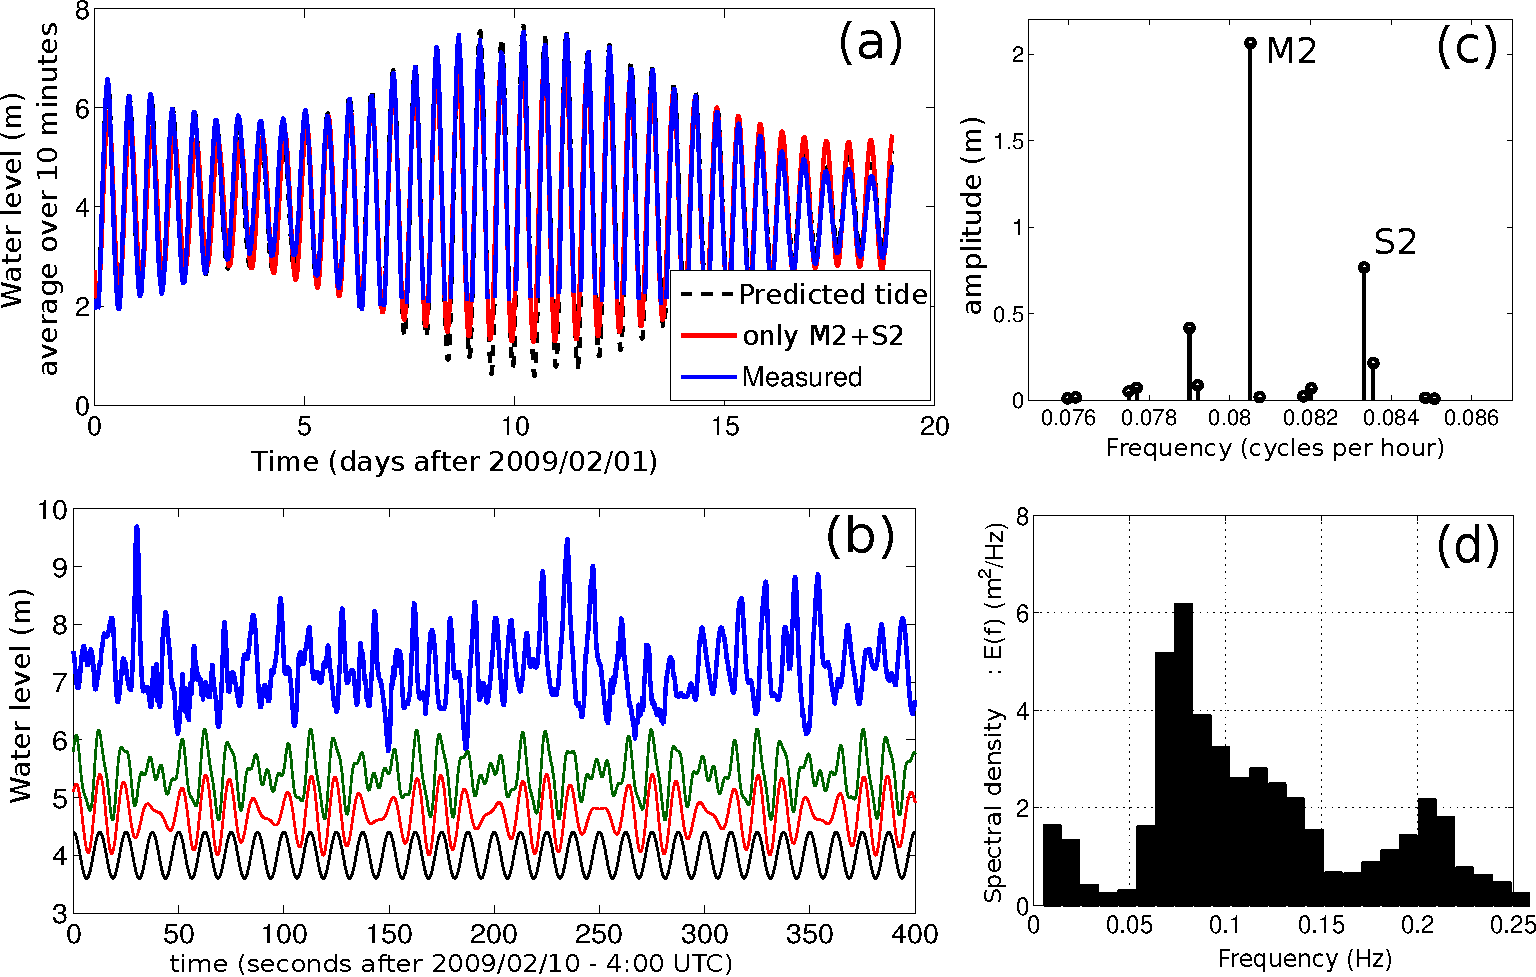
\includegraphics[width=\textwidth]{FIGS_CH_MEASUREMENTS/spectres_maree_vagues_en.pdf}}
%\vspace{3.64in}
  \caption{
Example of  surface elevation time series (a and b) deduced from pressure measurements collected 
as the foot of Western cliff of Banneg Island, Molene Archipelago. The corresponding spectra 
for the high and low frequency part illustrate the difference between a tide spectrum, 
presented as a function of amplitude and a wave spectrum. Below: a sample of the initial 
elevation signal and one, then two, then three sine waves are combined to approximate 
the initial signal. In the case of tides, the fit is already good with 2 components. In the case of 
waves, the detailed shape of the elevation cannot be reproduced without many components.}
\label{fig:maree_vagues}
\end{figure}
%%%%%%%%%%%%%%%%%%%%%%%%%%%%%%%%%%%%%%%%%%%%%%%%%%%%%%%%%%%%%%%%%%%%%%%%%
Figure \ref{fig:maree_vagues} shows how a tide elevation signal is already quite well 
reproduced by the superposition of only two sine waves (these two waves are called S2 and M2). 
On the contrary for the high frequency signal, dominated by waves, one, two or three sines 
waves (black, red and green) are far from sufficient for representing the initial signal (blue). 
Indeed, to reconstruct the wave signal a great number of sine waves with relatively close 
frequencies are required. For simplicity, let us start with one realization $m$ of an elevation 
time series, that can be expressed in terms of a Fourier series,
\begin{equation}
\zeta_{m}(t)=\sum_{i=1}^{N}a_{m,i}\cos(2\pi f_{i}t+ \Theta_{0,m,i})
\label{eq3.1}
\end{equation} 
Where $a_{m,i}$, $f_i$ and $\Theta_{0,m,i}$ are the Fourier amplitudes, frequencies and phases of 
the Fourier mode $i$, found for the realization $m$ of the sea state. As explained above, 
$N$ must be a large number. In practice the phases are nearly random and uniformly 
distributed over [$0,2\pi$] \footnote{The phases are not exactly random for an actual sea state, waves are 
slightly asymmetric, the front face being steeper than the back, and the crests sharper 
than troughs (e.g. \cite{Agnon&al.2005}). For most applications, these effects can be neglected.}. 
The ensemble mean of the Fourier amplitudes, expressed as function of the frequencies, 
 $A(f_i)= \left\langle a_{m,i}\right\rangle$ is called the amplitude spectrum.  For waves, 
identical sea state realizations can only be obtained in controlled laboratory experiments. 
Instead, the sea state is assumed stationary and the ergodicity theorem is evoked to replace the 
ensemble mean by a temporal mean. In practice, $M$ samples of a given (stationary) wave record simulate $M$ 
realizations of the sea state and provide an equivalent ensemble mean. 

For such random signals, the 'power' spectrum is preferred to the amplitude spectrum. 
As demonstrated in the previous chapter, the mechanical wave energy per unit surface of ocean, 
for an sine wave of amplitude $a$ is $\rho_w g a^2/2$. As a consequence, the energy spectrum is
\begin{equation}
\left\langle\frac{1}{2}a_{m,i}^{2}\right\rangle =\frac{1}{M}\sum_{m=1}^{M}\frac{1}{2}a_{m,i}^{2},
\label{eq3.2}
\end{equation}

With this definition, the values taken by the spectrum decrease proportionally to the spectral resolution $\Delta f$ that is the inverse of the length of time 
over which the spectral analysis is performed.  In order to avoid this dependency on the record length, it is customary to work with a power spectral density (PSD for short),
\begin{equation}
E(f_i)=\frac{1}{\Delta f} \left\langle \frac{1}{2} a_{m,i}^{2}\right\rangle. 
\label{eq3.3}
\end{equation}

In the limit of large record lengths, the frequency interval $\Delta f$ tends towards zero, and we obtain the continuous
wave energy frequency spectrum,
\begin{equation}
E(f)=\lim_{\Delta f\to 0}\frac{1}{\Delta f} \left\langle \frac{1}{2} a_{i}^{2}\right\rangle.
\label{eq3.4}
\end{equation}
 
While wave are irregular, the spectrum is relatively smooth, evolving slowly in space and time, with a typical time scale of a few hours. This regularity 
that contrasts with the apparent irregular motion of the sea surface, allows for a predictive numerical modeling. Note further, that
for convenience we continue to call (abusively) 'energy' the elevation variance $E$ which has units of length squared. 
The true energy, in Joules per unit surface, is in fact $\rho_w g E$. 

 This approach can be generalized to waves travelling in all directions. The Fourier representation of the sea surface elevation becomes,  
\begin{equation}
\zeta_m(x,y,t)=\sum_{i=1}^{N} \sum_{j=1}^{M}a_{m,i,j}\cos(2\pi f_{i}t- k_{i}\cos(\theta_{j}) x - k_{i}\sin(\theta_{j}) y + \Theta_{0,m,i,j}),
\label{eq3.5}
\end{equation}
as illustrated by figure \ref{fig:sumofsinewaves}
 %%%%%%%%%%%%%%%%%%%%%%%%%%%%%%%%%%%%%%%%%%%%%%%%%%%%%%%%%%%%%%%%%%%%%%%%%%%%%
\begin{figure}[!htbp]
\centerline{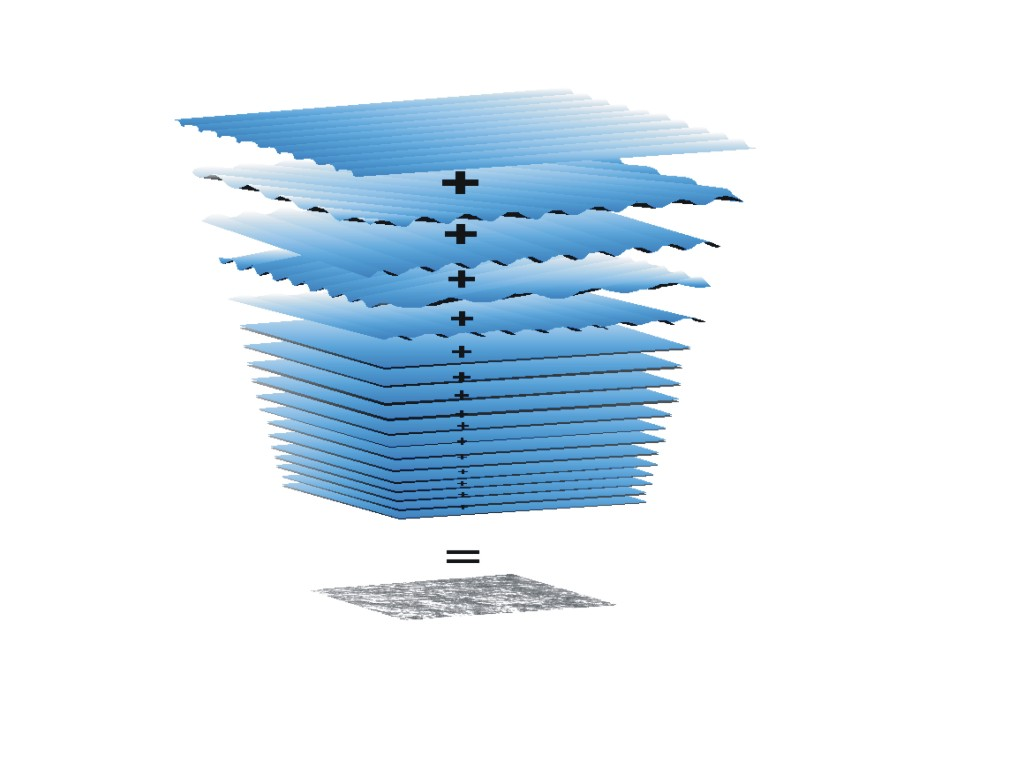
\includegraphics[width=0.8\textwidth]{FIGS_CH_MEASUREMENTS/Pierson1952.jpg}}
\caption{Reconstruction of a given sea state from the superposition of a great number of plane waves each with a particular direction and wavelength. Illustration of equation \ref{eq3.5}. 
After \cite{Pierson&al.1955}.\label{fig:sumofsinewaves}}
\end{figure}
 %%%%%%%%%%%%%%%%%%%%%%%%%%%%%%%%%%%%%%%%%%%%%%%%%%%%%%%%%%%%%%%%%%%%%%%%%%%%%

In this expression $k_{i}$ and $f_i$ are related by the linear dispersion relation and $\theta_{j}$ is the direction of
propagation of the Fourier mode ($i$,$j$). In the same fashion as for the frequency, the continuous frequency-direction wave energy
density spectrum, 
\begin{equation}
E(f,\theta)=\lim_{\Delta f\to 0}\lim_{\Delta \theta\to 0}\frac{1}{\Delta f \Delta \theta} \left\langle \frac{1}{2} \rho_w g a_{i,j}^{2}\right\rangle .
\label{eq3.6}
\end{equation}

Obviously, $E(f,\theta)$ is just a redistribution of $E(f)$ on the different wave directions and we recover the heave spectrum by summing on these directions, 
\begin{equation}
E(f) = \int_{0}^{2\pi}  E(f,\theta)d\theta.
\label{eq3.16}
\end{equation}

Keeping only the wave energy and its distribution reduces the   representation of the waves properties to a manageable amount of information, 
but some information is lost in the 
process. Indeed, it is not possible to reconstruct the sea surface from the spectrum, especially because the phases  are not conserved. 
In practice, the phase couplings are often negligible, and any reconstructed sea surface with 
random phases is statistically similar to the initial wave field. In this sense, for a Gaussian sea surface elevation, the spectrum contains 
the full statistics of the sea surface.

 \subsection{Wavenumber or frequency?}
 Depending on the measurement method, the numerical model or the application, one may want to perform the spectral analysis in the wavenumber or
 frequency space. The following relations between the frequency and wavenumber spaces, assume that waves follow the linear
 dispersion relation. The rule is simple, the variance of a given quantity does not depend on the coordinates in spectral space. 
The  variance is the spectral density times the spectral width, hence,
 \begin{equation}
E(f,\theta)d\theta df = E(k,\theta)d\theta dk 
\label{eq:Eftheta_Ektheta1}
\end{equation}
 which yields
 \begin{equation}
E(f,\theta)=\frac{\partial k}{\partial f} E(k,\theta) = \frac{2\pi}{C_g} E(k,\theta)
\label{eq:Eftheta_Ektheta}
\end{equation}

 In the same manner, 
 \begin{equation}
E(f,\theta)= \frac{2\pi}{C_g} E(k,\theta)= \frac{2\pi}{C_g}k E(k_{x},k_{y}) %=k\cos(f,k_{y})  CORRECT THIS !!!
\label{eq:Eftheta_Ekxky}
\end{equation}

The relationship must be used with caution for the high frequency part of the spectrum, because of nonlinear harmonics. This is significant at frequencies higher than three times the wind sea peak frequency \citep{Leckler&al.2015,Peureux&al.2018}. 
Finally, and we shall see why in chapter \ref{ch_current}, when the effects of currents on  waves are included, numerical models 
usually work with the action spectrum instead of the energy spectrum. This action spectrum is usually defined as 
 \begin{equation}
A(k,\theta)=\frac{1}{\sigma}E(k,\theta)=\frac{1}{\sigma}E(k_{x},k_{y})
\label{eq3.10}
\end{equation}
For instance, the numerical model WAVEWATCH III \citep{Tolman&Booij1998} calculates the evolution of $A(k,\theta)$ discretized over
 $N$ frequencies and $M$ directions, through the variable ASPEC(I,J) with $1 \leq I \leq N $ and $1 \leq J \leq M $. However, 
the model output is transformed back to $E(f,\theta)$.
 

%  \subsection{Some spectra}
 The spectrum is the primary variable of wave forecasting model, and, as such, it is important to be familiar with its physical meaning. 
 Figure \ref{fig:spectres101}
 illustrates the relation between the sea surface and spectrum shapes.
%%%%%%%%%%%%%%%%%%%%%%%%%%%%%%%%%%%%%%%%%%%%%%%%%%%%%%%%%%%%%%%%%%%%%%%%%%%%%
\begin{figure}[!htbp]
\centerline{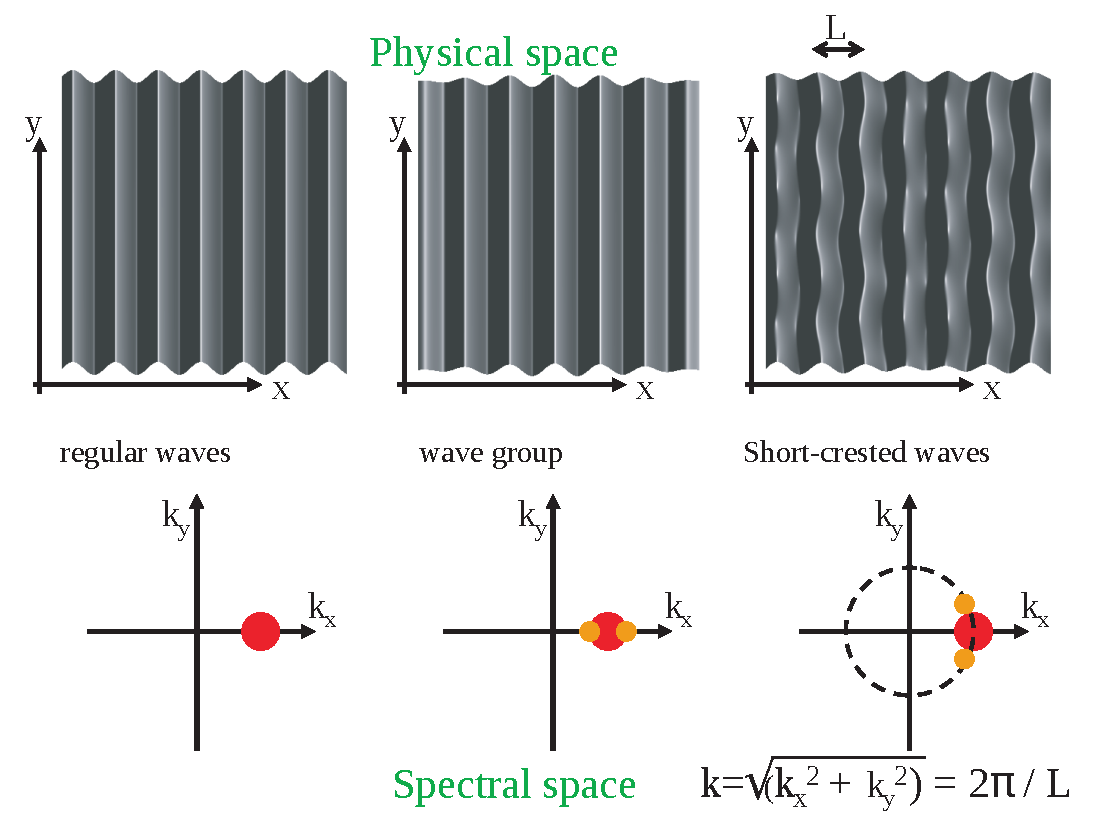
\includegraphics[width=0.8\textwidth]{FIGS_CH_MEASUREMENTS/spectres101_en.pdf}}
\caption{Relation between spectral and physical spaces. Schematic spectra of monochromatic waves (left panel) and modulated in terms 
of wavenumber or direction. For the last two cases, the surface is composed of three components.\label{fig:spectres101}}
\end{figure}
%%%%%%%%%%%%%%%%%%%%%%%%%%%%%%%%%%%%%%%%%%%%%%%%%%%%%%%%%%%%%%%%%%%%%%%%%%%%%
The reader is invited to try to recompose a sea surface in the physical space from the spectrum produced by a numerical model,
\begin{equation}
\zeta(x,y,t)=\sum_{m}^{M}\sum_{n}^{N}\sqrt{2E(f_m,\theta_n)\Delta_f \Delta_\theta} \cos\left[ k_m \cos \theta_n x +k_m \sin \theta_n  y- \sigma_m + \Theta_0(m,n)\right],
\label{eq3.11}
\end{equation}
where $\Delta_f$ and $\Delta_\theta$ are the spectral resolutions, and $M$ and $N$ are the number of frequencies and directions used to discretize the spectrum.  
Rigorously, $M$ and $N$ should be taken infinite, but we may start with the typical resolution of  a 
spectral wave model, of the order of 30 frequencies and 24 directions, with a significant level of energy in maybe only 20 components. If you want to get a more realistic surface it is best to interpolate the spectrum on a fine spectral grid, before taking the inverse Fourier transform. 

The component amplitude $\sqrt{2E(f_m,\theta_n)\Delta_f \Delta_\theta}$  is consistent with the fact that the total variance 
elevation is the sum of the amplitudes squared divided by two, or the spectrum integral over the entire spectral domain. 
The phase $\Theta_0(m,n)$ can be taken randomly distributed over [0,2$\pi$]. The resulting surface will look smoother than 
an actual sea state, and the observed crest-trough asymmetry will not be reproduced. This is due to the random phase assumption 
that disregards the phases coupling between spectral components. You may add some nonlinear effects with the "choppy" method, shifting your elevation map using an estimate of horizontal displacement, giving more realistic wave crest shapes \citep{Nouguier&al.2009}.  %These issues are further addressed in \S\ref{random_harmonics}.

\section{Using spectra}
Skipping here the technical details necessary for a practical estimation (see chapter \ref{ch_anaspec}), we now have a spectrum. Very nice, but what 
can we do with it? 

\subsection{Transfer function}\label{sub:transfer}
Depending on the application, one can transform the elevation variance spectrum. For a variable $A$ (for instance the bottom pressure), related to the  
surface elevation through a linear relation:
\begin{equation}
A=M\zeta,
\label{eq3.12}
\end{equation}
where $M$ is a complex number that takes values in the spectral space, the variance spectral density of $A$, $E_A$ is 
\begin{equation}
E_{A}(k_{x},k_{y})=|M|^{2}E(k_{x},k_{y})~\mathrm{or}~ E_{A}(f,\theta)=|M|^{2}E(f,\theta)
\label{eq:transfert}
\end{equation}
or any other equivalent expression in other spectral coordinates. For instance, the bottom velocity variance will be given from the polarization relation (\ref{polzeta})--(\ref{xi3}), that yield 
$M=\sigma \cos(\theta)/\sinh(kD)$, with $\theta$ the angle between the $x$-axis and the wave direction of propagation. We hence 
get the spectrum of the $x$-component of the bottom velocity.

Two of the most commonly used transfer functions are $M=\sigma$ for getting the surface orbital velocity magnitude in deep water, hence $M^2=4\pi^2 f^2$, and $M^2=\rho_w g/C_g=\rho_w g/(4 \pi f)$ for getting the energy flux in deep water. Using these transfer functions you get the surface orbital velocity variance 
\begin{equation}
<u^2+v^2>_{z=\overline{\zeta}}   =4\pi^2  \int_{0}^{\infty}  f^{2} E(f) {\mathrm d}f = 4\pi^2 m_2
\label{eq:moment_def}
\end{equation}
where $m_2$ is the second moment of the spectrum, and in general the  \textit{p-th} moment of the spectrum is defined as,
\begin{equation}
m_{p} = \int_{0}^{\infty}\int_{0}^{2\pi} f^{p} E(f,\theta)d\theta df
\label{eq:moment_def}
\end{equation}
Now, you may wonder why somebody would like to know the variance of the orbital velocity, well, it comes up, for example in Morison's equation that is the most widely used equation in offshore engineering to estimate forces on a structure \citep{Boccotti2000}, and other variances will matter for other applications. 

\subsection{Spectral and integral parameters: $H_s$, $T_p$ ...}\label{sub:param}
It can
be inconvenient  to describe a sea state by a two-variable function. Even when it is discretized into a numerical model,  typically 
over 30 frequencies and 24 directions meaning 720 spectral components, which is a lot of numbers to describe a sea state. This information can be 
summarized into a few meaningful parameters.

As the spectrum is a decomposition of sea surface variance, the most important parameter is certainly the variance $E$, often abusively called
energy. From the elevation variance $E$, we get a length scale  $\sqrt{E}$. Going back to sine waves, the variance is $a^2/2$ with $a$ the wave amplitude. Hence $\sqrt{2 E}$
is an equivalent amplitude  for random waves. More precisely, it is 
the root mean square amplitude. The root mean square wave height for a random wave is thus twice this amplitude
$H_{\mathrm{rms}}=2 \sqrt{2E}$.

For practical applications, the most widely used height scale is the \textit{significant wave height} $H_s$ that corresponds to the visual 
feeling given by the sea. From the wave height distribution we can define $H_{1/3}$ (see chapter \ref{ch1}). From the spectrum we define,
\begin{equation}
H_s \equiv H_{m0}\equiv 4 \sqrt{E} = 4 \sqrt{\int_{0}^{\infty} E(f) {\mathrm d}f}
\label{eq3.14}
\end{equation}
In practice $H_{m0} \simeq H_{1/3}$, this property can be demonstrated in the limit of a narrow spectrum \citep{Longuet-Higgins1952}. Following the recommendations of 
the World Meteorological Organization, 
we shall consider $H_{m0}$ to be \emph{the} definition of the significant wave height $H_s$. The "$m0$" index indicates that it is based on the zeroth moment of the spectrum. 


In many cases, the directional information is not available, and we only have the frequency spectrum $E(f)$. 
This distribution of the energy as a function of frequency contains information on the typical time scales of the signal. $E(f)$ generally exhibits 
a sharp maximum around the frequency $f_p$, $E(f_{p})=E_{\max}$. $f_p$ is the peak frequency, corresponding to the peak period $T_{p}=1/f_p$.  
This peak period can be noisy in the presence of several peaks, as in Fig. \ref{fig:Hawaii_spectrum}.
The frequency distribution can also be characterized from the spectral moments, $m_p$, 
\begin{equation}
T_{m0,p} =  \left[m_p/m_0\right]^{-1/p} \simeq \left[\left(\int_{0}^{f_{\max}} f^{p} E(f) df\right)/\left({\int_{0}^{f_{\max}} E(f) {\mathrm d}f}\right)\right]^{-1/p}.
\label{eq3.17}
\end{equation}
The most widely used periods are $T_{m0,-1}$, $T_{m0,1}$, $T_{m0,2}$. Each of these has more or less weight on low frequency part of the spectrum.
If one is interested in an effect proportional to $f^2$, as is  the case of the wave forces exerted on a structure, it is reasonable to use $T_{m0,2}$.
Besides, $T_{m0,2}$ is very close to the mean period $T_z$ given by  wave-by-wave analysis. Note however that in practical calculations, $T_{m0,2}$ depends on the choice
of $f_{\max}$. The values of the different periods for a typical spectrum are shown in figure 
\ref{fig:Hawaii_spectrum}.
%%%%%%%%%%%%%%%%%%%%%%%%%%%%%%%%%%%%%%%%%%%%%%%%%%%%%%%%%%%%%%%%%%%%%%%%%%%%%%%%%%%%%
\begin{figure}[htb]
\centerline{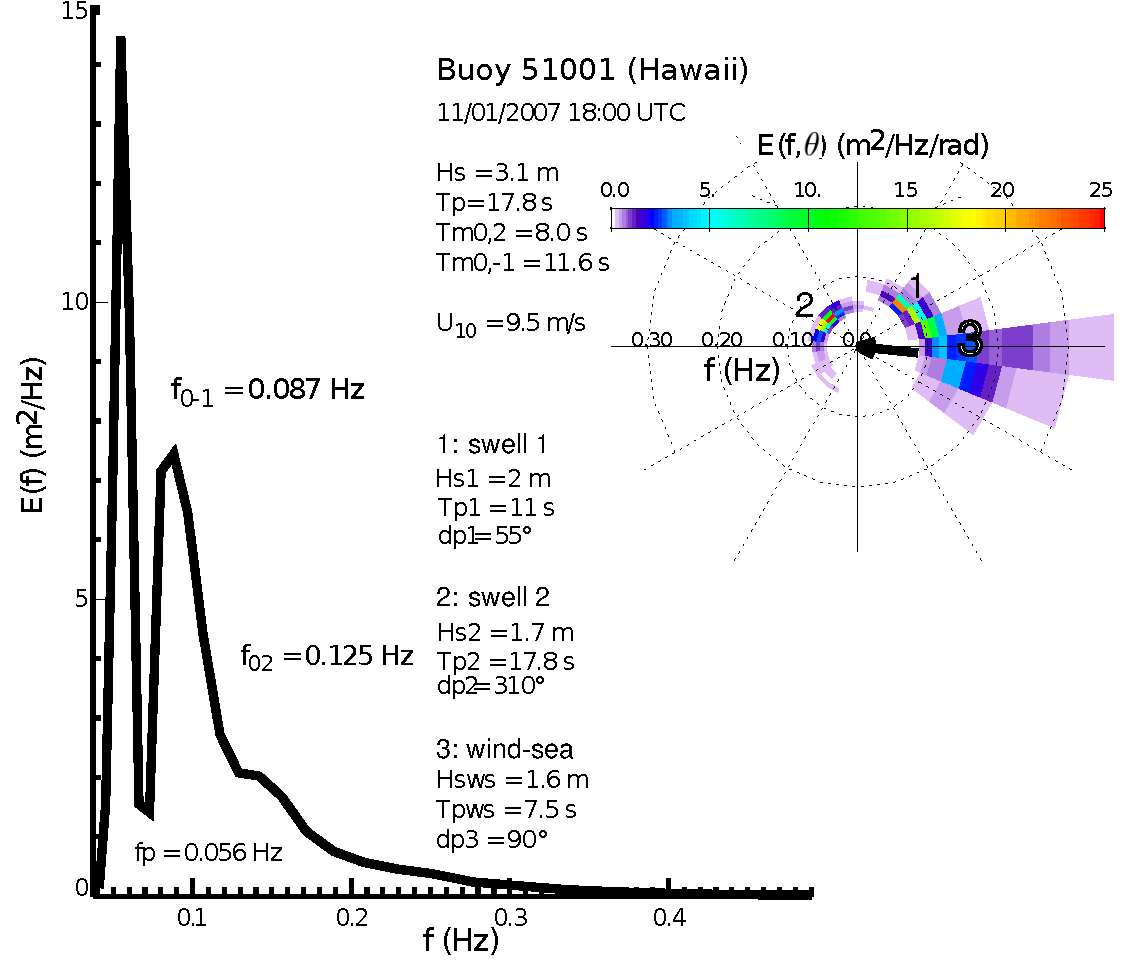
\includegraphics[width=0.7\textwidth]{FIGS_CH_MEASUREMENTS/exemple_spectre_Hawaii.pdf}}
\caption{
Typical example of a oceanic spectra in tropical area, measured by buoy 51001, moored 350 km North West of Kauai island, on January 11, 2007. 
The different peak and mean periods are indicated along with the parameters produced by a decomposition of the spectrum into a primary
swell, secondary swell and wind sea. This analysis is generally not possible without directional information. Note that the wind sea only appears 
as a soft "shoulder" to the right of the secondary swell, while it comes from a different direction. This shows the possible difficulty of 
separating swell and wind sea from a frequency spectrum. Also note that the significant 
wave height $H_s$ is less than the sum of $H_{s1}$, $H_{s2}$, $H_{sws}$, of the three systems: the energy can be summed but the wave heights cannot.
Namely $H_s=\sqrt{H_{s1}^2+H_{s2}^2+H_{sws}^2}$.}
\label{fig:Hawaii_spectrum}
\end{figure}
%%%%%%%%%%%%%%%%%%%%%%%%%%%%%%%%%%%%%%%%%%%%%%%%%%%%%%%%%%%%%%%%%%%%%%%%%%%%%%%%%%%%%%%%%%%


Finally, we define, 
\begin{eqnarray}
a_{1}(f) & = &\int_{0}^{2\pi} \cos{\theta} E(f,\theta)d\theta /\int_{0}^{2\pi} E(f,\theta)d\theta, \label{a1def} \\
b_{1}(f) & = & \int_{0}^{2\pi} \sin{\theta} E(f,\theta)d\theta /\int_{0}^{2\pi} E(f,\theta)d\theta ,\label{b1def} 
\end{eqnarray}
that can be estimated from the elevation spectrum $E(f)$ and the elevation-horizontal displacements
co-spectra, $E_{xz}$ and  $E_{yz}$, as detailed in chapter \ref{ch_anaspec},   eqs. (\ref{Exz})--(\ref{Eyz}). 

The mean wave direction at frequency $f$ is, 
\begin{equation}
\theta_{m}(f)=\arctan(a_{1}(f)/b_{1}(f)),
\label{eq3.20}
\end{equation}
and the directional spreading, as defined by \cite{Kuik&al.1988} is the standard deviation (in radians) of the spectral width
in the limit of a narrow spectrum,
\begin{equation}
\sigma_{\theta}(f)=\left[2(1-(a_{1}^{2}(f)+b_{1}^{2}(f))^{1/2}) \right]^{1/2}.
\label{eq3.21}
\end{equation}
For equal energies in opposite directions, $\sigma_{\theta}$ is maximum at 
$\sqrt{2}$ radians, which is $81\,^{\circ}$. 

The directional wave properties of the dominant waves, can also be characterized with the 
mean direction and directional spreading of the spectral peak: $\theta_{m}(f_{p})$ and $\sigma_{\theta}(f_{p})$. 
$\theta_{m}(f_{p})$ is often referred to as "main direction", while the mean direction would rather be an average
over the entire spectrum,
\begin{equation}
\theta_{M}(f)=\arctan \left(\int_{0}^{\infty} b_{1}(f) E(f)df/\int_{0}^{\infty} a_{1}(f) E(f)df\right)
\label{eq3.22}
\end{equation}
With all these directions, one must be careful with the directional convention. The directions are usually counted
from North (direction 0), progressing clockwise (90 east, 180 south, 270 West). However, depending on the authors, the direction convention is either meteorological (direction
from where the waves or wind are coming, this is the convention used in the present manuscript) or oceanographic convention
(direction toward which the waves or currents are moving). Be careful!

 

 \section{Random waves \textit{in situ} observations}
 The most common usage of wave time series is the determination of the frequency spectrum $E(f)$ and, when more than 
 one variable are measured, the directional wave spectrum $E(f,\theta)$ may be estimated. Details of this processing 
 given in chapter \ref{ch_anaspec}. In practice, the most common in situ 
 instruments for wave measurements are surface-following buoys or bottom-mounted pressure gauges or ADCPs.  
 
 \subsection{Wave gauges}
 These are reference sensors that directly measures the free surface elevation $\zeta(x,y,t)$ at a fixed horizontal position $(x,y)$. 
 The measure is done through the 
electrical resistance or capacity of one (or two) conducting wires forming a loop closed by the sea surface. This type of sensor is widely 
used in the laboratory, but it is not so common at sea because this requires a fixed  platform
 and the wires are susceptible to damage by small floating debris. Also, the large wave heights encountered in the field require long 
 enough gauges. These wave 
gauges can also be mounted on a buoy that filters out the long waves through its motion \citep{Graber&al.2000}. Wave gauges are most often 
associated in an array (see below) of several gauges synchronized and mounted on a single platform so as to 
provide a wave direction estimation \citep{Cavaleri&al.1981}.

The direct measurement of surface elevation can also be performed by radar and LIDAR systems, which determine the  
distance to the sea surface from the travel time of an electromagnetic or sound wave, and that can likewise be arranged in an fixed array or integrated 
in a scanning system.


  \subsection{Wave buoys}
    Buoys measure either the successive positions and velocities, determined by a global navigation satellite system (such as the Global Positioning System - GPS) or 
    vertical acceleration recorded by a buoy floating at the free surface that give after a double integration in time, 
  a surface elevation signal $\zeta(x,y,t)$. Depending on the type of instrument and on the presence of currents, the horizontal position $(x,y)$ is not fixed but 
  nearly follows the wave orbital 
motion. This later property may be annoying for purists of the wave profile, as it partly filters out the free surface nonlinearity (the linear 
Lagrangian motion involves a part of the nonlinear Eulerian motion). In addition to the heave measurement, that was for long the most common, the wave 
direction can be determined by measuring the horizontal accelerations that yields, through double integration, the horizontal displacement $x$ 
and $y$ (figure \ref{Datawell_xyz}). 
\begin{figure}
\centerline{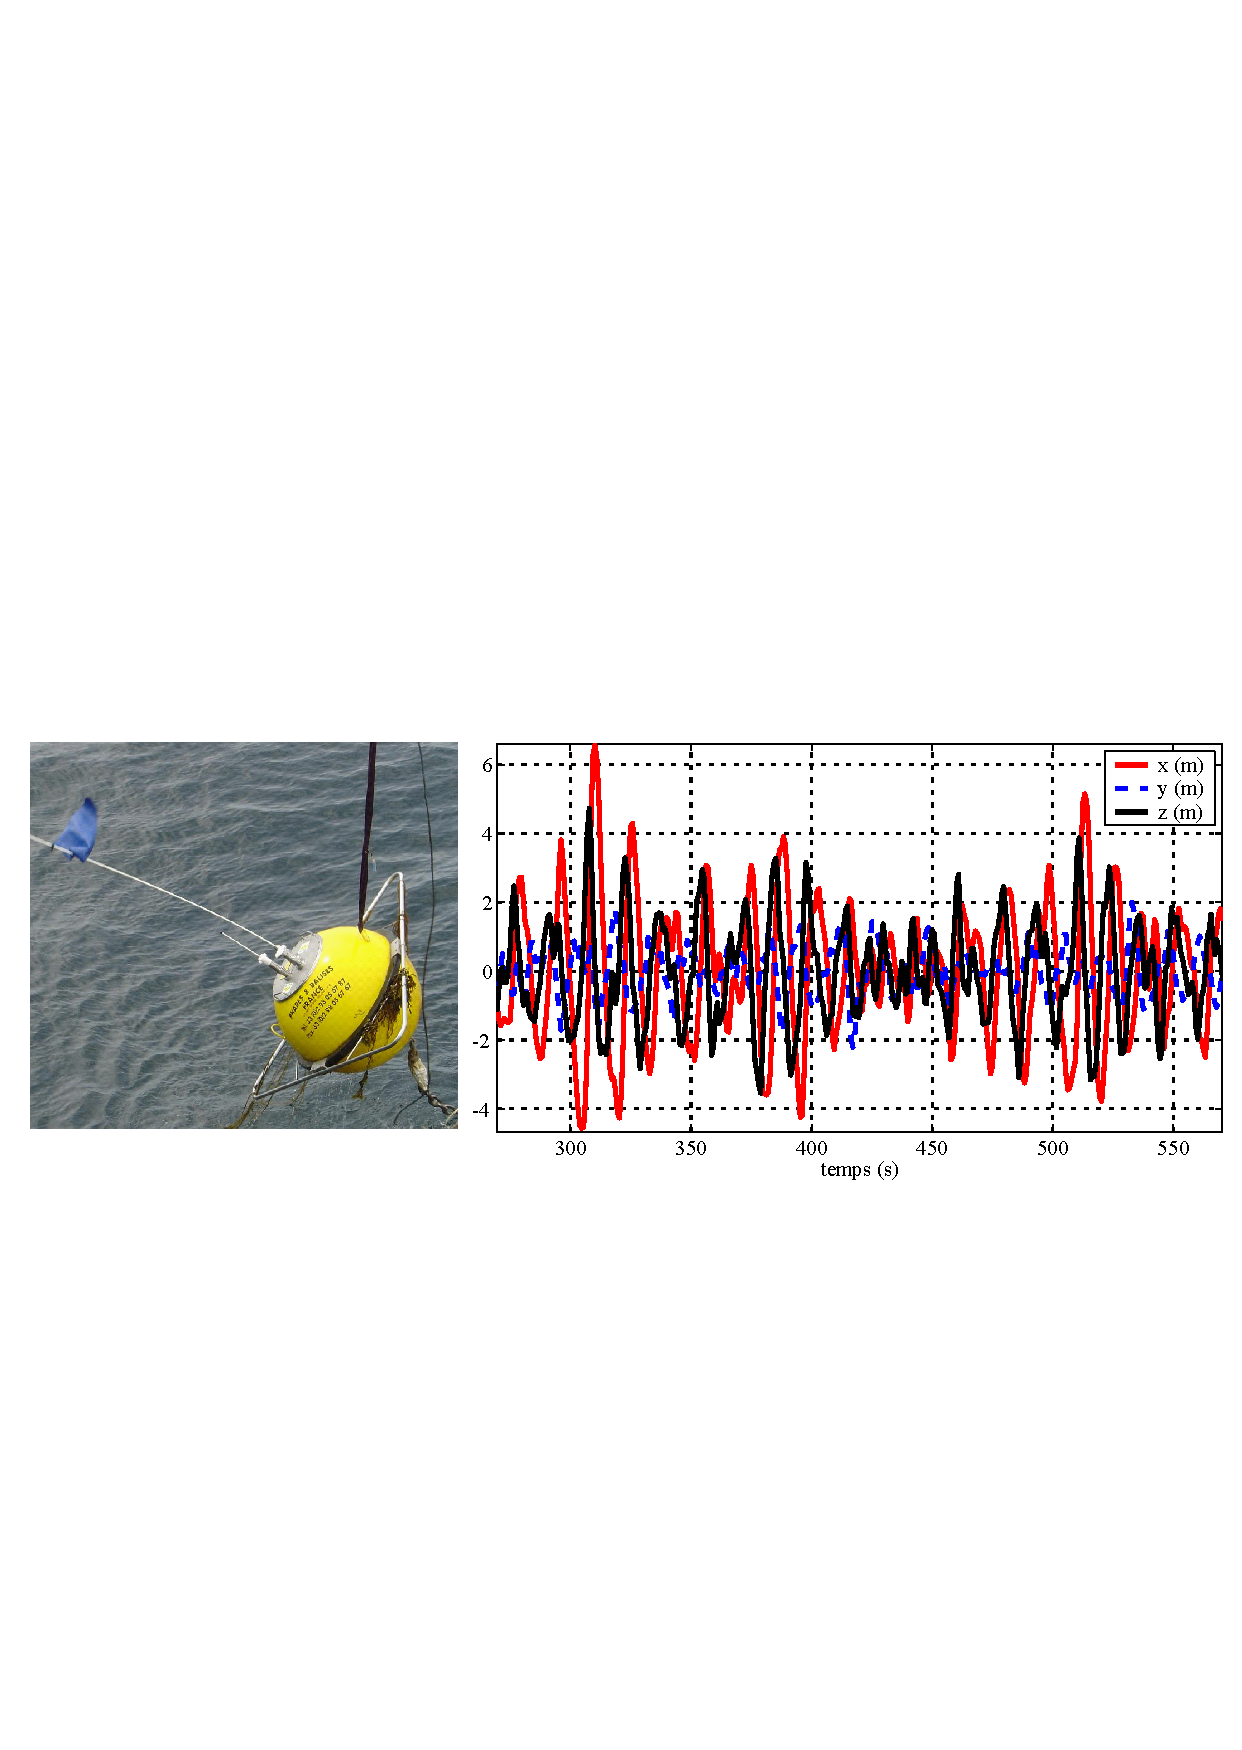
\includegraphics[width=\textwidth]{FIGS_CH_MEASUREMENTS/Exemple_DWIROISE2004all_plus.pdf}}
\label{Datawell_xyz}
\caption{Left panel: Deployment of a  Datawel Waverider buoy, 0.9 m of diameter, equipped with a (long) HF radio antenna and 
with a (short) Orbcomm satellite antenna for data transfer. Right panel: examples of displacements measured by this buoy offshore Crozon in May 2004. 
(same time series as in figure \ref{FigWaveriderTSz}). Of course, the 10~m high waves were not measured by the times of the buoy deployment.}
\end{figure}
 The use of  precise satellite positioning now allows a direct measure of the 3-component position and velocity, the latter being generally more accurate \citep{Herbers&al.2012}. Many companies have commercialized such buoys.

The largest buoys generally use a measurement of the components $\partial \zeta /\partial x$ and $\partial \zeta/ \partial y$ and of the local free 
surface slope: pitch and roll as the first prototypes of \cite{Longuet-Higgins&al.1963} and \cite{Cartwright&Smith1964}. This is the case of the US 
National Data Buoy Center (NDBC) 3-m diameter buoys.
Details of buoy processing are given in chapter \ref{ch_anaspec}. Both methods, acceleration and pitch-roll allow, thanks to the three signal covariance, 
the determination of the first four Fourier coefficients 
of the angular distribution, also known as angular moments,
\begin{itemize}
  \item  $a_1$ and $b_1$, defined by (\ref{a1def})--(\ref{b1def}) and calculated from the co-spectra $E_{xz}$ and $E_{yz}$ (equations \ref{Exz}--\ref{Eyz})
\item $a_2$ and $b_2$, defined as $a_1$ andf $b_1$ but with $\cos \theta$ and $\sin \theta$ replaced by $\cos 2 \theta$ and $\sin 2 \theta$, respectively.
\end{itemize}

A more complete measure of the directional spectra from floating buoys has been developed but has not been as successful as expected: the cloverleaf buoy that consists in three 
pitch-roll buoy linked to each other \citep{Mitsuyasu&al.1975}. In principle this layout provides a measure of the surface curvature and the Fourier coefficient up to $a_8$ and $b_8$.
From a conventional buoy, one has to infer the function $S(f,\theta)$ from only the four independent number $a_1$, $b_1$, $a_2$ and $b_2$. This is not so much a 
measurement problem, but rather one of choosing a statistical estimator. There are many method for this. Among these, the Maximum Entropy Method \citep[MEM][]{Lygre&Krogstad1986}, 
has the advantage of conserving the angular moment  $a_1$, $b_1$, $a_2$ and $b_2$. The MEM method tends however to 
to give a bimodal shape (two-peak spectra), which is often \citep{Ewans1998} but not always realistic \citep{Benoit&al.1997}.

Other recent analysis techniques aim at increasing the the directional resolution of this kind of measurements. For instance, \cite{Donelan&al.1996}, 
have proposed an interesting method based on a wavelet transform. Unfortunately their method assumes that for any given frequency 
the wave field is dominated by waves coming for one single direction, which is not the case. This analysis yields a very high directional resolution, and can be interesting 
to detect the presence of waves from a given direction, but it cannot be interpreted as a directional spectrum as it leads to a low bias in the directional spreading. Other methods can be biased and 
should be avoided. This is 
the case of the maximum likelihood method (MLM) which yields output spectra that are systematically too broad and have moments $a_1$, $b_1$, $a_2$ and $b_2$ that 
are different from the input parameters.
 
 \subsection{Pressure gauges}
 When surface elevation measurements are too expensive or not possible, which may be due to strong currents incompatible with mooring lines, breaking waves in the surf zone, a usually good alternative is the measurement from bottom-mounted sensors. The most common and robust are pressure gauges that can be used to measure 
 tidal elevations at the same time. To recover the surface elevation from the pressure signal, we can invert the linear transfer function given by eq. (\ref{pression}), 
 namely, for a sensor at a height $h_d$ over the bottom,  $M=\rho_w g \cosh(kh_d)/\cosh(kD)$, with $k$ estimate from the frequency $f$ of each spectral component of the time series, using the Airy wave dispersion relation. In shallow water and for waves of large amplitudes, this method often underestimates the wave height because the linear dispersion is not very accurate \citep{Filipot&al.2010,Bonneton&Lannes2017}. The water depth $D$ is also given by the measurement of 
 the mean pressure once it is corrected for the atmospheric pressure. Because the elevation to pressure transfer function $M$ decreases when  $k$ increases, it is usually impossible to recover  wave elevations for frequencies above a cut-off value $f_c$. That value $f_c$ is a function of water
 depth, instrument noise, background noise (usually due to currents), but also of the directional wave spectrum. Indeed, figure \ref{fig:pressure_with_2ndorder}
 shows an example of data recorded in 100~m depth, in which the second order pressure is larger than the linear pressure for frequencies above 0.13~Hz. As discussed in part 3, 
 this second order spectrum is a function of the frequency spectrum $E(f)$ but also of the directional wave distribution. In that case, it is not possible 
 to recover $E(f)$ for frequencies above 0.12~Hz. For example, on day 4, the yellow-orange sloping line at frequencies 0.05 to 0.1 Hz is 
 a due to swell waves arriving from a distance of about 4000~km (see explanations in chapter \ref{ch3}, eq. (\ref{prev lin1})). 
 At the same time, there is a fainter blueish line at twice these frequencies which is caused by the 
 second order effect. The vertical blue stripes above 0.13~Hz are caused by the tidal current effects on the directional wave spectrum \citep{Ardhuin&al.2013}.
 %%%%%%%%%%%%% figure
\begin{figure}[htb]
\centerline{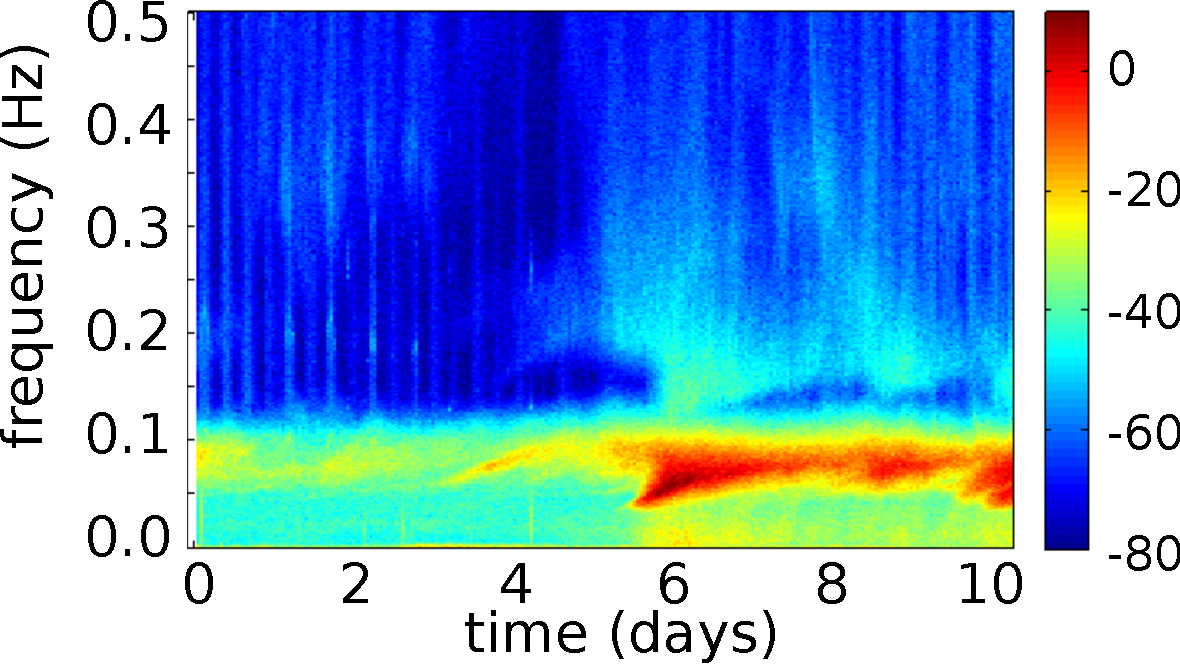
\includegraphics[width=0.7\textwidth]{FIGS_CH_MEASUREMENTS/pressure_with_2ndorder.pdf}}
%\vspace{3.64in}
  \caption{Bottom pressure spectra}
    {Time-frequency diagram of the pressure recorded over 11 days in 100~m depth off the French Atlantic coast in October 2015.  The colors show the pressure level in dB relative 
    to 1~m$^2$/Hz times $\rho_w^2 g^2$. These measurements were performed by a very sensitive Paroscientific piezo-electric sensor, included in a RBR-duo 
    system, with a noise level below -80 dB. At our depth of 100~m, the usual linear pressure signal, with a level between -40 to 10 dB, can be used to recover 
    the surface elevation spectrum for frequencies below 0.12~Hz. At higher frequencies, the pressure is dominated by a second order effect due 
    to waves in opposite directions \citep[e.g.][]{Miche1944b,Ardhuin&al.2013}. That effect has very important consequences for seismology, as discussed in part 3.} \label{fig:pressure_with_2ndorder}
\end{figure}
%%%%%%%%%%%%% end of figure

 
\subsection{P-U-V sensors}
As indicated by its name, this sensor measures the pressure $p$ and the two horizontal components of the velocity, $u$ and $v$. It is indeed the 
combination of two instruments: a current meter (acoustic, electromagnetic because a high sampling rate is required) and a pressure sensor, often 
piezo-electric. This instrument is of particular interest as it is designed to be installed on the sea bottom. It is the simplest mooring you may imagine, if one 
is not too worried about fishermen, for instance. Of course, it is difficult ut not impossible to recover real time data (cables, acoustical modems with surface buoys...).

We have seen in Chapter 2 that the fluid pressure and velocities exponentially decay from the surface to the bottom with a typical scale which correspond 
to the wave length 2$\pi/k$. The "P-U-V" sensor is thus perfect if one wish to measure the agitation at the bottom. To measure the wave heights one may use
the theory that provide transfer functions between pressure, velocities, elevation, etc (equation \ref{eq:transfert}). In this situation, the closer to 
the surface, the more reliable will be the measurement (e.g. an instrument mounted on a floating of fixed platform).

 \subsection{Sensor arrays and ADCPs}
A set of wave gauge can be combined to record more covariances between the measurements. This kind of 
measure allowed to get the first accurate spectra \citep{Donelan&al.1985} and is particularly used for the air-sea interaction studies, 
for which the short waves spectrum is crucial \citep{Graber&al.2000, Pettersson&al.2003}. It is essential to synchronize the sensors with 
an accuracy that is small compared to the measured wave period. Similar techniques are employed in RADAR and SONAR technologies to determine the sources of echoes. The original array processing algorithms 
used for waves were actually developed for seismology.

 These techniques have been largely applied to pressure sensors arrays with a number of statistical methods for the spectrum estimation 
 \citep[e.g.][]{Davis&Regier1977, Long&Hasselmann1979, Pawka1983, Herbers&Guza1990}. An example of a spectrum is given in Figure \ref{wave spectra} 
determined from a coherent array of pressure sensors deployed in 8m depth on the site of the US Army Corps Field Research at Duck, North Carolina. 
For large arrays, the underwater instruments positioning much be very accurate. An acoustical positioning is generally used.
%%%%%%%%%%%%% figure
\begin{figure}
\centerline{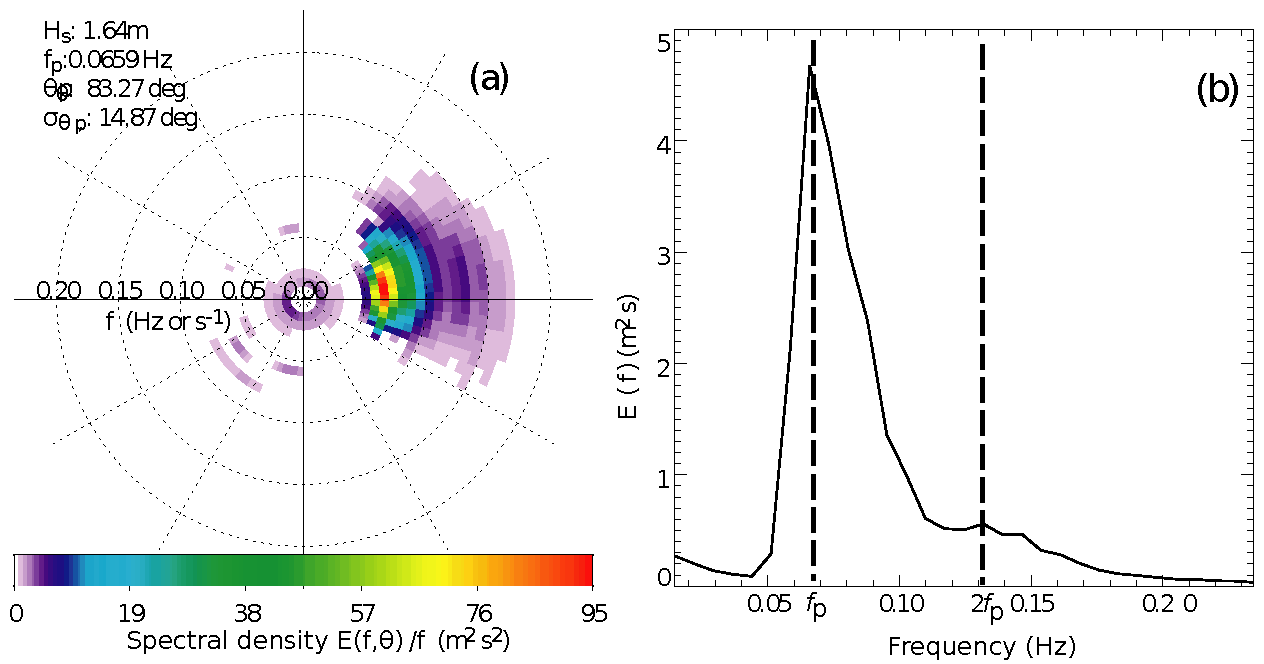
\includegraphics[width=0.6758\textwidth]{FIGS_CH_MEASUREMENTS/introduction_fig1.pdf}}
\caption{(a) Example of frequency-direction wave spectra, divided by frequency, computed from 8m depth pressure measurements in Duck, NC, October 
19, 1994, 7:00 (EST). (b) Corresponding Frequency spectra whose secondary peak matches the first harmonic of the spectral peak 
($f=2f_p$), and which is likely due to the effect of nonlinear interactions that are of great importance in shallow water.}
\label{wave spectra}
\end{figure}
%%%%%%%%%%%%% end of figure
  The directional resolving power of the array generally increases with the number of sensors in the array \citep[see][]{Kinsman1965}. 
  Arrays of pressure sensors are excellent reference instruments for measuring the spectra of dominant waves,  but they 
are relatively expensive to deploy and maintain. \cite{OReilly&al.1996} used such an array for the validation of directional properties of two different types of 
buoys. %However, comparisons have shown that for the parameters estimated from the the moments  $a_1$, $b_1$, $a_2$ and $b_2$, 
%the Datawell wave buoy, for instance, gives excellent results \citep{OReilly&al.1996}. Sensors arrays get useful only when further details on the 
%wave spectra are required (separation of incident and reflected waves, or of different wave systems, etc...). 

A recent and convenient alternative is the use of current profilers (ADCP).  The combination of the velocities measured by different acoustic beams, 
allows, in principle, for an interesting measure of the directional spectra. However, the typical noise of up-looking ADCPs does not allow a 
higher angular resolution than that of a simple P-U-V \citep{Herbers&Lentz2010}. The main benefit of ADCPs, however, is the use of measurements close to the sea surface, 
where the wave motion is less attenuated than at the bottom. 

\section{Optical measurements}
Waves are usually the first thing that you see when looking at the sea. But turning beautiful pictures into numbers for scientific analysis is 
not so easy. We will not discuss here the techniques that are mostly used in the laboratory (e.g. light refraction across the air-sea interface), but 
instead we present the main methods in use for application to real ocean waves. 
\subsection{From stereo-photography to stereo-video}
The first methods used to measure wave shapes were based on stereo-photography: pairs of photographs taken at the exact same time can be analyzed to 
produce a 3D map of the sea surface \citep{Schumacher1939}. The basic principle is to determine the $(x,y,z=\zeta(x,y))$ coordinates of points that have been 
identified in both images. This identification can be done using automatic correlation analysis. The pair of pictures can be obtained from a single platform to cover a modest area and reveal interesting 
details about the wave shapes \citep{Banner&al.1989}, typically less than 30 by 30~m, 
or from a pair of aircraft to get a view of a much broader region \citep{Cote&al.1960,Holthuijsen1983b} and produce a full directional 
wave spectrum. 
%%%%%%%%%%%%%%%%%%%%%%%%%%%%%%%%%%%%%%%%%%%%%%%%%%%%%%%%%%%%%%%%%%%%%
\begin{figure}[htb]
  \center{\noindent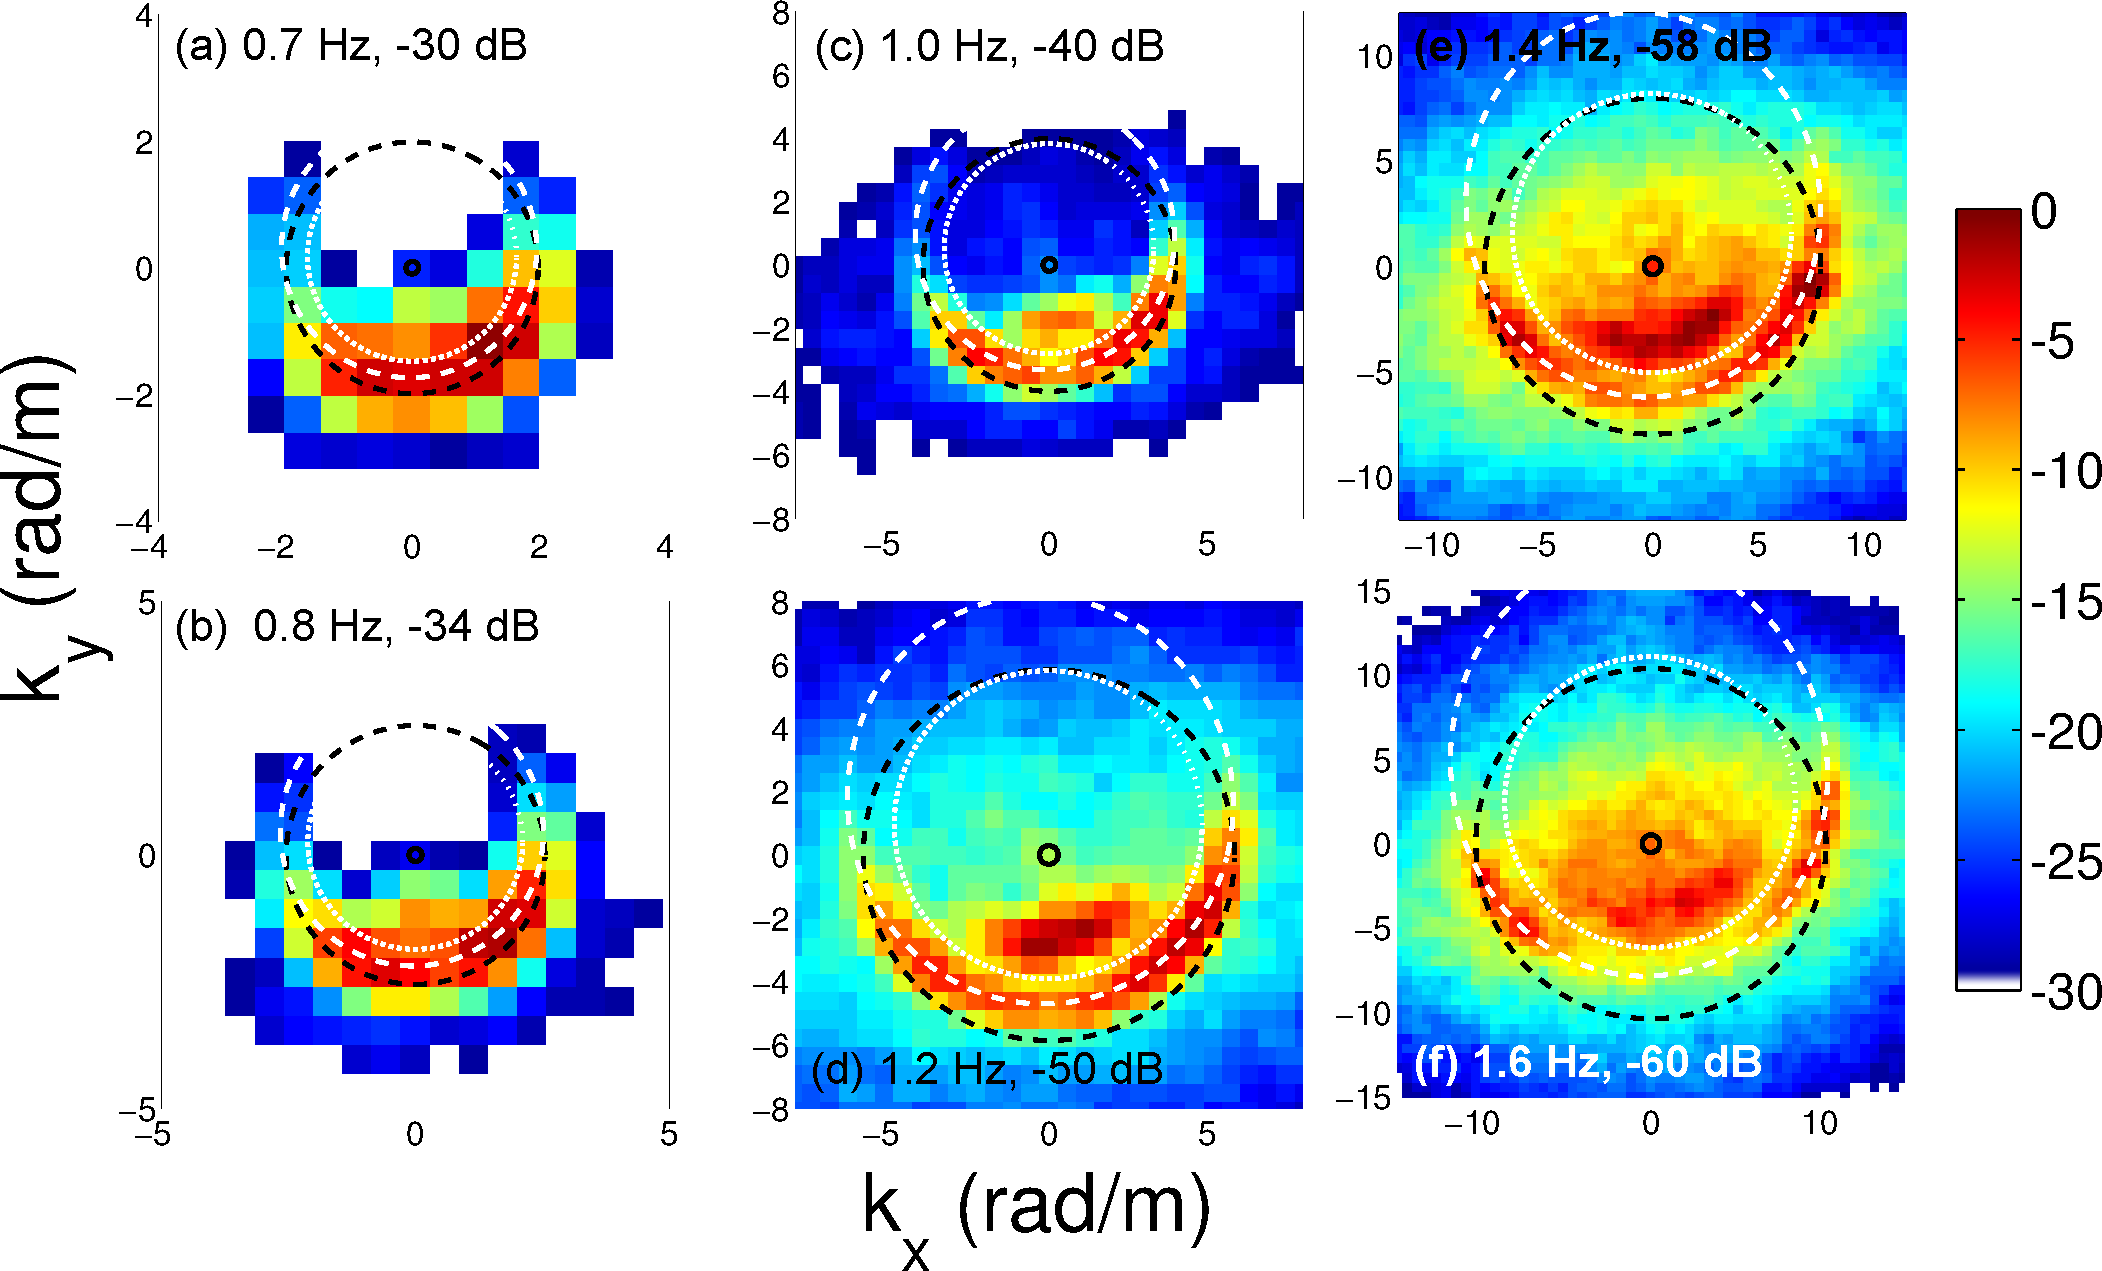
\includegraphics[width=0.8\linewidth,angle=0]{FIGS_CH_MEASUREMENTS/kxky_spec1_nosmooth.pdf}}\\
  \caption{Slices of the double-sided spectrum for positive apparent frequencies 0.7, 0.8, 1.0, 1.2, 1.4 and 1.6 Hz. The energy appears in the direction from 
           where it is coming. For each panel the color scale spans 30 dB with the dark red corresponding to the power indicated on 
the figure (e.g. -30 dB) relative to 1~m$^4$/Hz. Note that 1.4 and 1.6 Hz are twice 0.7 and 0.8 Hz, so that the first harmonic of the components in (a) and (b) 
           appear at approximately twice the wavenumbers in panels (e) and (f). In each panel, the linear dispersion relation without current is plotted in black, and the  white dashed line gives the linear dispersion with a uniform current $U= 0.15$ m/s oriented towards the trigonometric angle 99 degrees. The white dotted  line marks approximately the separation between 
the linear part of the spectrum and the faster non-linear components (Adapted from Leckler et al. 2015). } \label{fig:kxky}
\end{figure}
%%%%%%%%%%%%%%%%%%%%%%%%%%%%%%%%%%%%%%%%%%%%%%%%%%%%%%%%%%%%%%%%%%%%%
Now that everyone is carrying a digital camera around, and that stereo processing is much more common, there are many opportunities 
to measure the full evolution  of the sea surface in space and time $\zeta(x,y,t)$. Recent efforts by \cite{Benetazzo2006} and \cite{Gallego&al.2011} 
have demonstrated the capabilities of stereo processing, leading to new applications \citep{Fedele&al.2013,Leckler&al.2015}. Latest developments include  
auto-calibration and the proper motion corrections needed for ship deployments. A general issue that remains is that not all light conditions are favorable. Alternatively, the use of 
more expensive infrared cameras or polarization cameras is a very interesting extension for overcoming the variability of lighting conditions and 
the lack of texture at small scale 
for a correlation analysis \citep{Sutherland&Melville2013,Laxague&al.2015}.

The great advantage of having the full surface $\zeta(x,y,t)$, is that we can now measure a 3D spectrum, without the need to use linear wave theory. 
This is most important for the short wave components, for which nonlinear contributions are important. Figure \ref{fig:kxky} shows slices of the 3D spectrum 
at a constant frequency. These are obtained from a stereo-video system installed 11~m above the water in a platform in the Black Sea. The image processing 
uses the epipolar method: the position of the sea surface is obtained only by a knowledge of the geometry of the camera system.
This record from October 4, 2011, was acquired when the wind speed was 14~/s and the wave  peak frequency is $f_p=0.33$~Hz \citep{Leckler&al.2015}. The 
Non-linear contributions to the frequency spectrum dominate for $f > 4 f_p$. For example at $f=1.2$~Hz, there is more energy in the peak located near $(k_x=0,k_y=-3)$ 
than along the linear dispersion relation shown wit the white dashed line. 
Such non-linear effects are also important for the statistics of extreme wave heights, as shown by \cite{Fedele&al.2013} and \cite{Benetazzo&al.2017}.



\subsection{Using polarization and/or light intensity}
Such a stereo system has difficulties in measuring waves with frequencies higher than 1.4~Hz that have small heights. Other measurement techniques that 
are directly sensitive to slopes are better suited for these shorter components: these include polarimetry \citep{Zappa&al.2008} or a measurement of 
the radiance that can also be combined with the epipolar method \citep{Gallego&al.2011,Yurovskaya&al.2013}. 

Such a technique can also be applied to high resolution airborne or satellite imagery (with pixel sizes less than 30~m in order to resolve waves). 
\cite{Kudryavtsev&al.2017} have particularly taken advantage of the O(1~s) time lag in the acquisition of the different color channels of the Multi Spectral Instrument 
on board Sentinel-2. Clouds or haze obviously limit the application of optical methods, which is why radar is often preferred for wave remote sensing. 


\subsection{Grazing angle radar}
 Rotating radars are usually deployed at the coast, for ship traffic monitoring, or on ships, for navigation safety, providing a detection of ships, land, and sea ice. 
  Most of these radar work in X-band, with a wavelength around 3~cm, but S-band can also be used. These radars also record many echos from the sea surface due to waves.  This `sea clutter' is another case of the saying, \emph{somebody's noise is somebody else's signal}. 
 The clutter greatly limits the detection of ships at sea, but wave and current information can be extracted from it \citep{Young&al.1985}.
%%%%%%%%%%%%% figure
\begin{figure}[htb]
\centerline{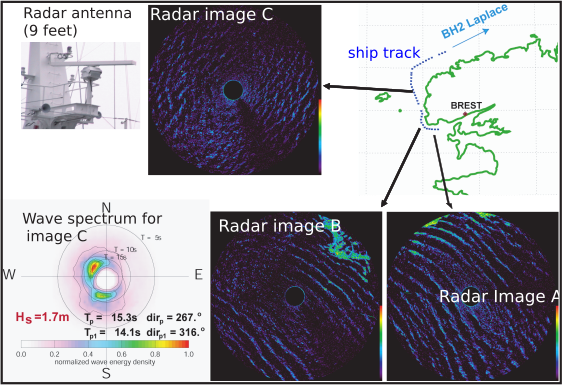
\includegraphics[width=0.73\textwidth]{FIGS_CH_MEASUREMENTS/wamos_en.png}}
\caption{Examples of radar images recorded with a grazing radar (WAMOS system, Oceanwaves GmbH), onboard the Hydrographic vessel Laplace. The measurements
were undertaken in March 2003, with a very long and high  swell from the West ($H_{s}=6$~m, $T_{p}=26$~s). The spectrum shown here was obtained in the shadow of Ouessant.
The swell go around the islands. At the ship location part of the energy has been refracted and arrives from the south.}\label{wamosfig}
\end{figure}
%%%%%%%%%%%%% end of figure
 Because of the low elevation afforded from a ship, the incidence angle of radar waves on the sea surface is grazing. Hence, the sea surface exhibits shadows behind wave crests and 
 the relationship between the backscatter image and the sea surface is fairly nonlinear. Still, the wave spectrum may be related to the radar image spectrum using 
 a transfer function (figure \ref{wamosfig}). The analyses procedure uses
a sequence of several images, in order to decrease the noise. The 3D (frequency-wavenumber-direction) spectrum is estimated to filter the data into 'wave patterns'  that follow 
the linear gravity wave dispersion relation, and other echoes and noise. This kind of system generally
gives a good spectral energy distribution, but the gain (proportionality factor between the radar image spectrum 
and the surface elevation spectrum) is not very accurate,  leading to typical errors of 20\% or more on the estimate of $H_s$. 
An additional measurement form an altimeter, or a motion sensor giving heave or pitch/roll from a ship, can provide an independent
measure of this gain. In systems that allow a measurement of the Doppler signal \citep[e.g.][]{Farquharson&al.2005}, the orbital velocities may be measured, but the radar really 
measures the velocities of scatterers which -- at this incidence -- contains also the phase velocities of steep waves.
A side-product of the dispersion relation analysis is are maps of surface currents, with sub-kilometer resolution, and water depth if the water is shallow enough.  This is probably the best instrument available today  for the measurement of sub-mesoscale currents over a footprint of about 10~km in diameter. A full exploitation of the dispersion relation can also provide an estimate of the vertical current shear near the surface \citep{Lund&al.2015}. 

\subsection{Surface wave radar}
An extreme case of grazing angle occurs when the radar waves propagate along the surface. This kind of propagation is possible
in the HF-VHF range (from 2 to 50 MHz). This surface wave allows indeed to get information beyond the horizon. 

%%%%%%%%%%%%% figure
\begin{figure}[htb]
\centerline{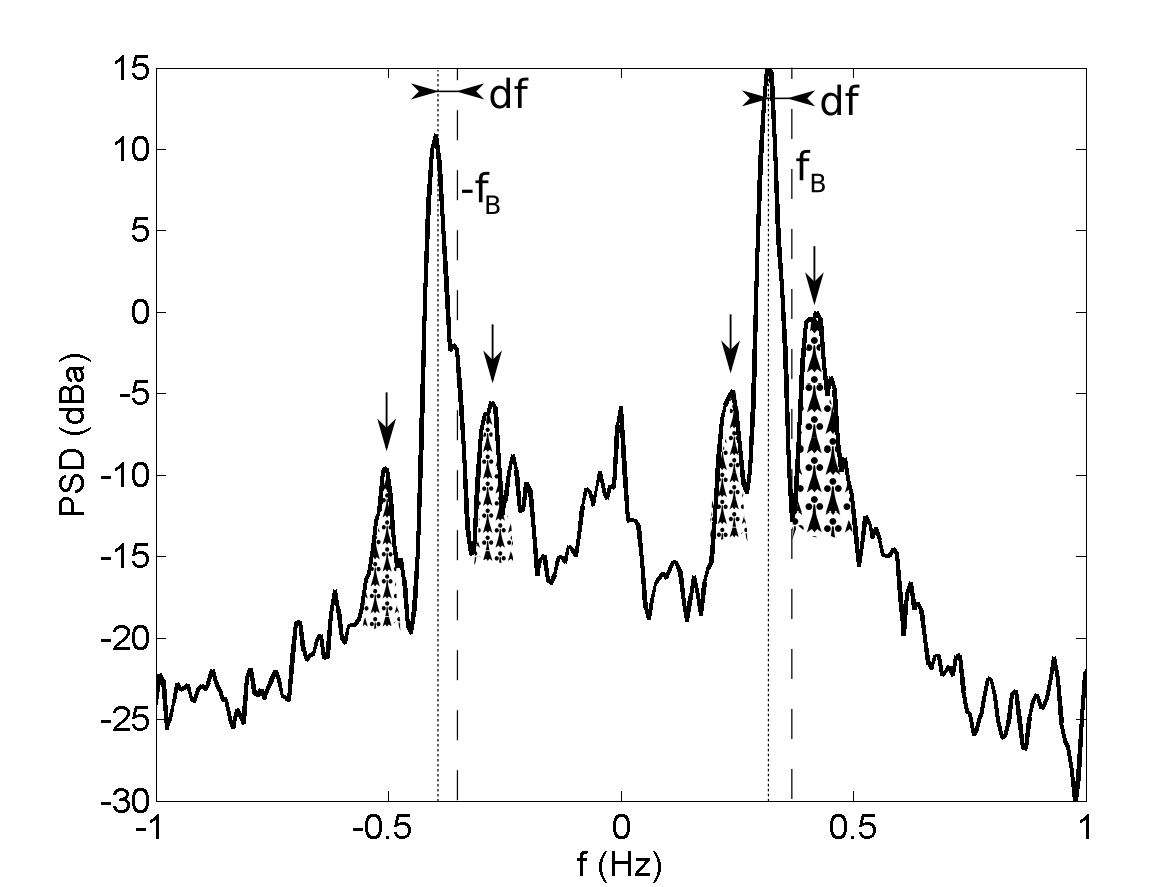
\includegraphics[width=0.5\textwidth]{FIGS_CH_MEASUREMENTS/Spectre_bin_10_touch.png}}
%\vspace{3.64in}
  \caption{Example of Doppler spectrum from a HF radar.}{This measured spectrum comes from the Porspoder radar (Finistere, France). 
The radar frequency is 12.4~MHz, corresponding to a wavelength $L_e=2 \pi/k_e=24$~m. The main echoes is due to Bragg scattering, 
which selects the ocean waves with a wavelength $L_e/2=12$~m that propagate towards ($f > 0$)  or away from the radar ($f<0$). 
Multiple scattering by waves with wavenumbers  $\kb_1$ and $\kb_2$, such that $2 \kb_e = \kb_1 + \kb_2$
gives the 'second order echoes'. At first order, i.e. for linear waves, the waves of wavenumber $k_w=2 k_e$ 
have a frequency $f_B=\pm \sqrt{g 2 k_e} =\pm 0.36$~Hz  in deep water. The anomaly $df$ of the two highest peaks in the Doppler spectrum 
indicate that the phase speed $2 \pi f / k$ is different from the linear wave theory without current. 
the main reason for that difference is usually the presence of a current, with a velocity $U_r=2 \pi df / (2 k_e)$ in the direction of the radar. }\label{HFspectrum}
\end{figure}
%%%%%%%%%%%%% end of figure

The radar reflection is well explained by Bragg theory, with the maximum backscatter power at the Doppler frequency $f_D$ occuring for 
electromagnetic incident and reflected wave numbers vectors $\kb_i$ and $\kb_r$ that match with the wavenumber $\kb_w = \pm \kb_i \mp \kb_r$ 
and and the wave frequency $f_D=f$, where $f$ and $\kb_w$ are related by the linear dispersion relation. 
In the monostatic configuration where the receiving and transmitting antenna are almost at the same place, we have $\kb_i = \kb_e$,  $\kb_r= - \kb_e$, 
and $\kb_w = 2 \kb_2$. 

The observed Doppler spectrum can be
interpreted as the superposition of simple reflections (or first order reflections) and multiple reflections. 
The extraction of sea state spectra is possible from the second order that is a convolution of the spectrum 
\citep[see for instance][]{Wyatt2000}. These second order echoes are weaker than first order echoes at Bragg frequencies. The main echoes are used for currents measurement. Their frequency provides a measurement of the Bragg wave phase velocity. The deviation 
of this phase velocity from the expected linear wave phase speed can be interpreted as a surface drift current \citep{Ardhuin&al.2009b}. 
This current includes non-linear corrections to the phase velocity, which is like a filtered Stokes drift \citep{Stewart&Joy1974,Broche&al.1983,Ardhuin&al.2009}.
The secondary peaks are caused by either the multiple reflection of radar waves, or the single reflection off nonlinear wave components. 
In some cases a peak can be seen at the frequency $\sqrt{2}f_B$ which corresponds to the reflection from the first harmonic of waves with wavenumber 
$\kb = \pm \kb_e$, which have a frequency, $2\sqrt{g k_e}$ in deep water. Because different wave components have different sensitivities to the current profile, 
it is possible to use that peak to measure the vertical shear of the current \citep{Ivonin&al.2004}. 


%\section{The limitations to the usual wave spectrum}
%The spectrum gives the full statistical properties of waves, provided the components are effectively independent. Yet, this is not exactly true as waves are slightly nonlinear. Two main relations exist between components: the presence of harmonics and modulations. The first effects comes from the fact that a single nonlinear wave train corresponds to several spectral components whose wave number and frequency are multiple of that of the carrier wave. Rigorously speaking, one needs the 3D spectrum $E(f, \mathbf{k})$ to discern these harmonic waves that do not follow the linear dispersion  (Figure \ref{fig:kxky}). The 3D spectrum estimation requires specific instruments, mapping the surface in space and time. The link between the  3D spectrum and the linear part of the spectrum is the topic of ongoing research. The calculation technique of dressed and undressed spectrum presented by  \cite{Elfouhaily&al.2003}  is a possible approach: the undressed spectrum corresponds to the linear part and the dressed part to the nonlinear spectral contents. To lowest order, however, the full spectrum  can be obtained by the second order correction \citep{Janssen2009,Leckler&al.2015}. 

%The modulation effect is a bit more complex. Typically, short waves in the presence of much longer waves see their environment modified. In particular, the apparent gravity felt by short waves is the standard gravity plus the vertical acceleration induced by the longer waves motion. In the same fashion, the long waves orbital velocities acts as a variable current on the short waves.  These effects are one of the likely causes of the higher breaking rate of short  waves at the crest of long waves \citep{Dulov&al.2002,Guimaraes2018}. The short wave spectra is hence modulated by the long waves. In practice, for the wind sea, such effects are weak for waves with frequency less that three times the peak frequency \citep{Banner&al.1989}. This factor 3 on the frequency corresponds to a factor 10 on the wavelength (in deep water).

%Modulations can be caused by other effects than the presence of other waves. In particular, if the medium in which the wave propagate is not homogeneous, then the wave field will contain wavelengths that are interferences between the medium and the waves, and that do not correspond to the linear dispersion relation.  These non-homogeneities can be variations in water depth, current, gravity, surface tension ... 

%If these modulations occur  at scales similar to the wavelength, besides the local effect on the waves there is also a scattering of the waves with the generation of waves in other directions, frequencies, or other types of waves, such as the Bragg scattering  caused by underwater topography that is described in chapter \ref{ch5}, or the generation of seismic waves over a sloping bottom in  chapter \ref{chsismo}. These scattering effects result in an evolution of the spectrum in space and time. 

%If the scales are shorter than the wavelength, then the medium is a 'meta-meterial', which 
%can exhibit funny properties like negative refraction indices and can be used to create 'invisibility shields'. Although 
%these effects can be created in the laboratory, they may not be relevant for ocean waves, due to 
%the random nature of waves and the generally irregular patters in geophysical 
%contexts.
